\chapter{Related Work}
\label{cha:RelatedWork}

Public transportation navigation apps help commuters plan, track and complete their journeys more efficiently. 
While many apps provide route tracking, the challenge of knowing exactly when to get off at the right stop persists for passengers.
Without clear alerts, passengers must constantly monitor their route which can be inconvenient or impractical, especially in unfamiliar areas.

This chapter examines three popular transit apps and how they handle user alerts for exiting public transportation.
While all three apps provide detailed navigation and tracking, their approaches to stop notifications differ.
Some rely on Live Activities for glanceable updates on the lock screen while others offer explicit stop alerts.

\section{Google Maps}
Google Maps was developed by Google and is a mapping service that offers route planning across different transportation modes including driving, walking, cycling and public transit. 
The platform has partnered up with numerous public transportation providers globally to integrate their data while also collecting information independently to facilitate trip planning for users.
Google Maps provides real-time transportation information that allows users to view live arrivals for buses, metros and subway systems and alerts them to canceled routes.
According to 9to5Google \cite{google_maps_live_activity}, Google Maps began testing the Live Activities feature on iPhones in 2023 to enable users to receive navigation updates directly on their lock screens and in the Dynamic Island. 
Live Activities offer glanceable directions, estimated time of arrival and upcoming turns without the need to unlock the device.
However, only a limited number of users have reported seeing this feature appear intermittently while navigating with Google Maps.
Figure~\ref{fig:GoogleMaps} (left) shows Google Maps' route planning and detailed tracking in Figure~\ref{fig:GoogleMaps} (middle). 
The Live Activity feature, also referred to as "Glanceable Directions" by Google, can be toggled in the settings but appears inconsistently with no known way to manually enable it. 
When it activates automatically, it appears as shown in Figure~\ref{fig:GoogleMaps} (right).

\begin{figure}[htbp]
    \centering
    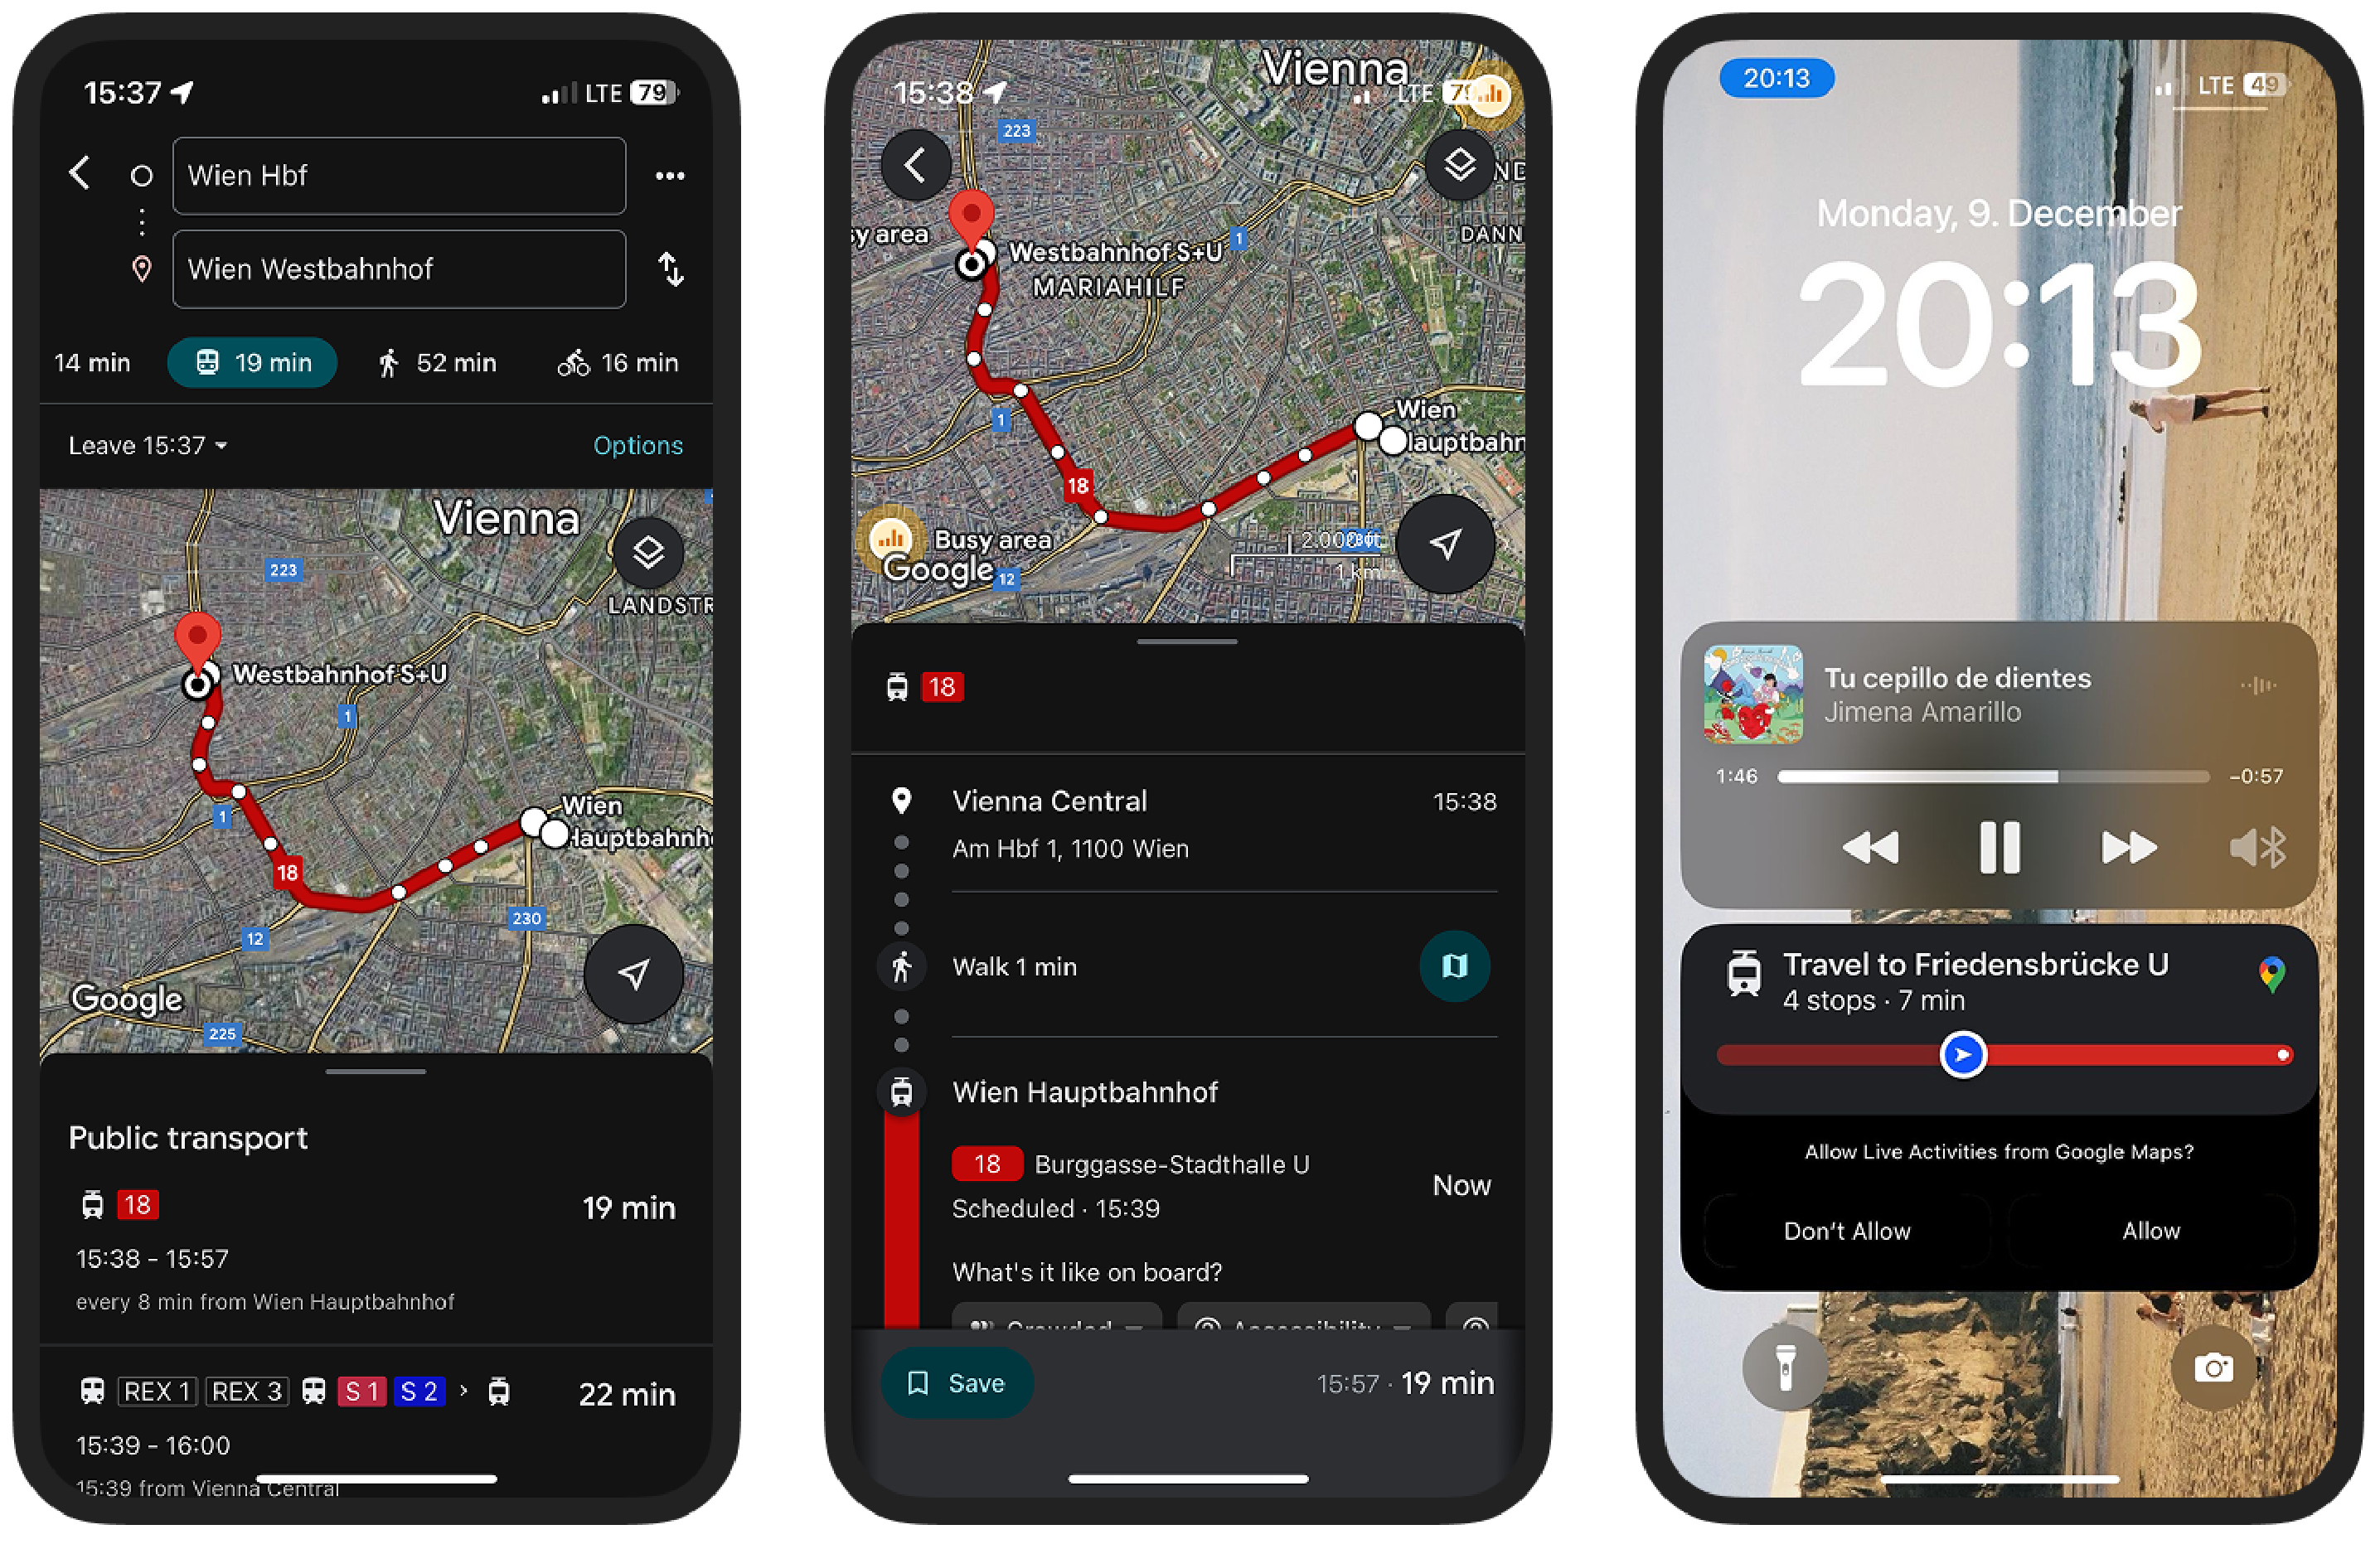
\includegraphics[width=0.7\textwidth]{GoogleMaps.pdf}
    \caption{Public transport route planning in the Google Maps app (left) and its Live Activity feature (right)}
    \label{fig:GoogleMaps}
\end{figure}

\section{Citymapper}
Citymapper was founded in 2011 by former Google employee Azmat Yusuf, who aimed to simplify navigation for London's public transport system, as highlighted by TechRound \cite{citymapper_profile}.
The app was initially launched as Busmapper and focused on London's bus network.
Over time, it expanded to include the underground, trams and other transport modes and eventually became Citymapper.
Today, the platform operates in over 100 cities worldwide including New York, Paris, Tokyo, Vienna and Sydney, according to their website \cite{citymapper_cities}.
Additionally, it supports entire regions like Scotland, the Basque Country and the Balearic Islands.

The app uses real-time data from multiple transit services to provide route planning and live tracking.
It suggests the fastest and most convenient routes while considering delays and disruptions and offers users the possibility to receive notifications for service alerts.
Furthermore, users are notified when approaching their designated stops if they enable this feature, as stated on their website \cite{citymapper_getoffalerts}.
Since iOS 16.1, Citymapper introduced Live Activities allowing users to follow the progress of their trip without unlocking their iPhone, as stated on Citymapper's Website \cite{citymapper_ios_lock_screen_navigation}.
Figure~\ref{fig:Citymapper} (left) shows Citymapper's route planning. 
When "Go" is pressed in the detailed navigation in Figure~\ref{fig:Citymapper} (middle) and the user is near the route, the Live Activity starts and displays real-time trip progress on the lock screen as in Figure~\ref{fig:Citymapper} (right).

\begin{figure}[htbp]
    \centering
    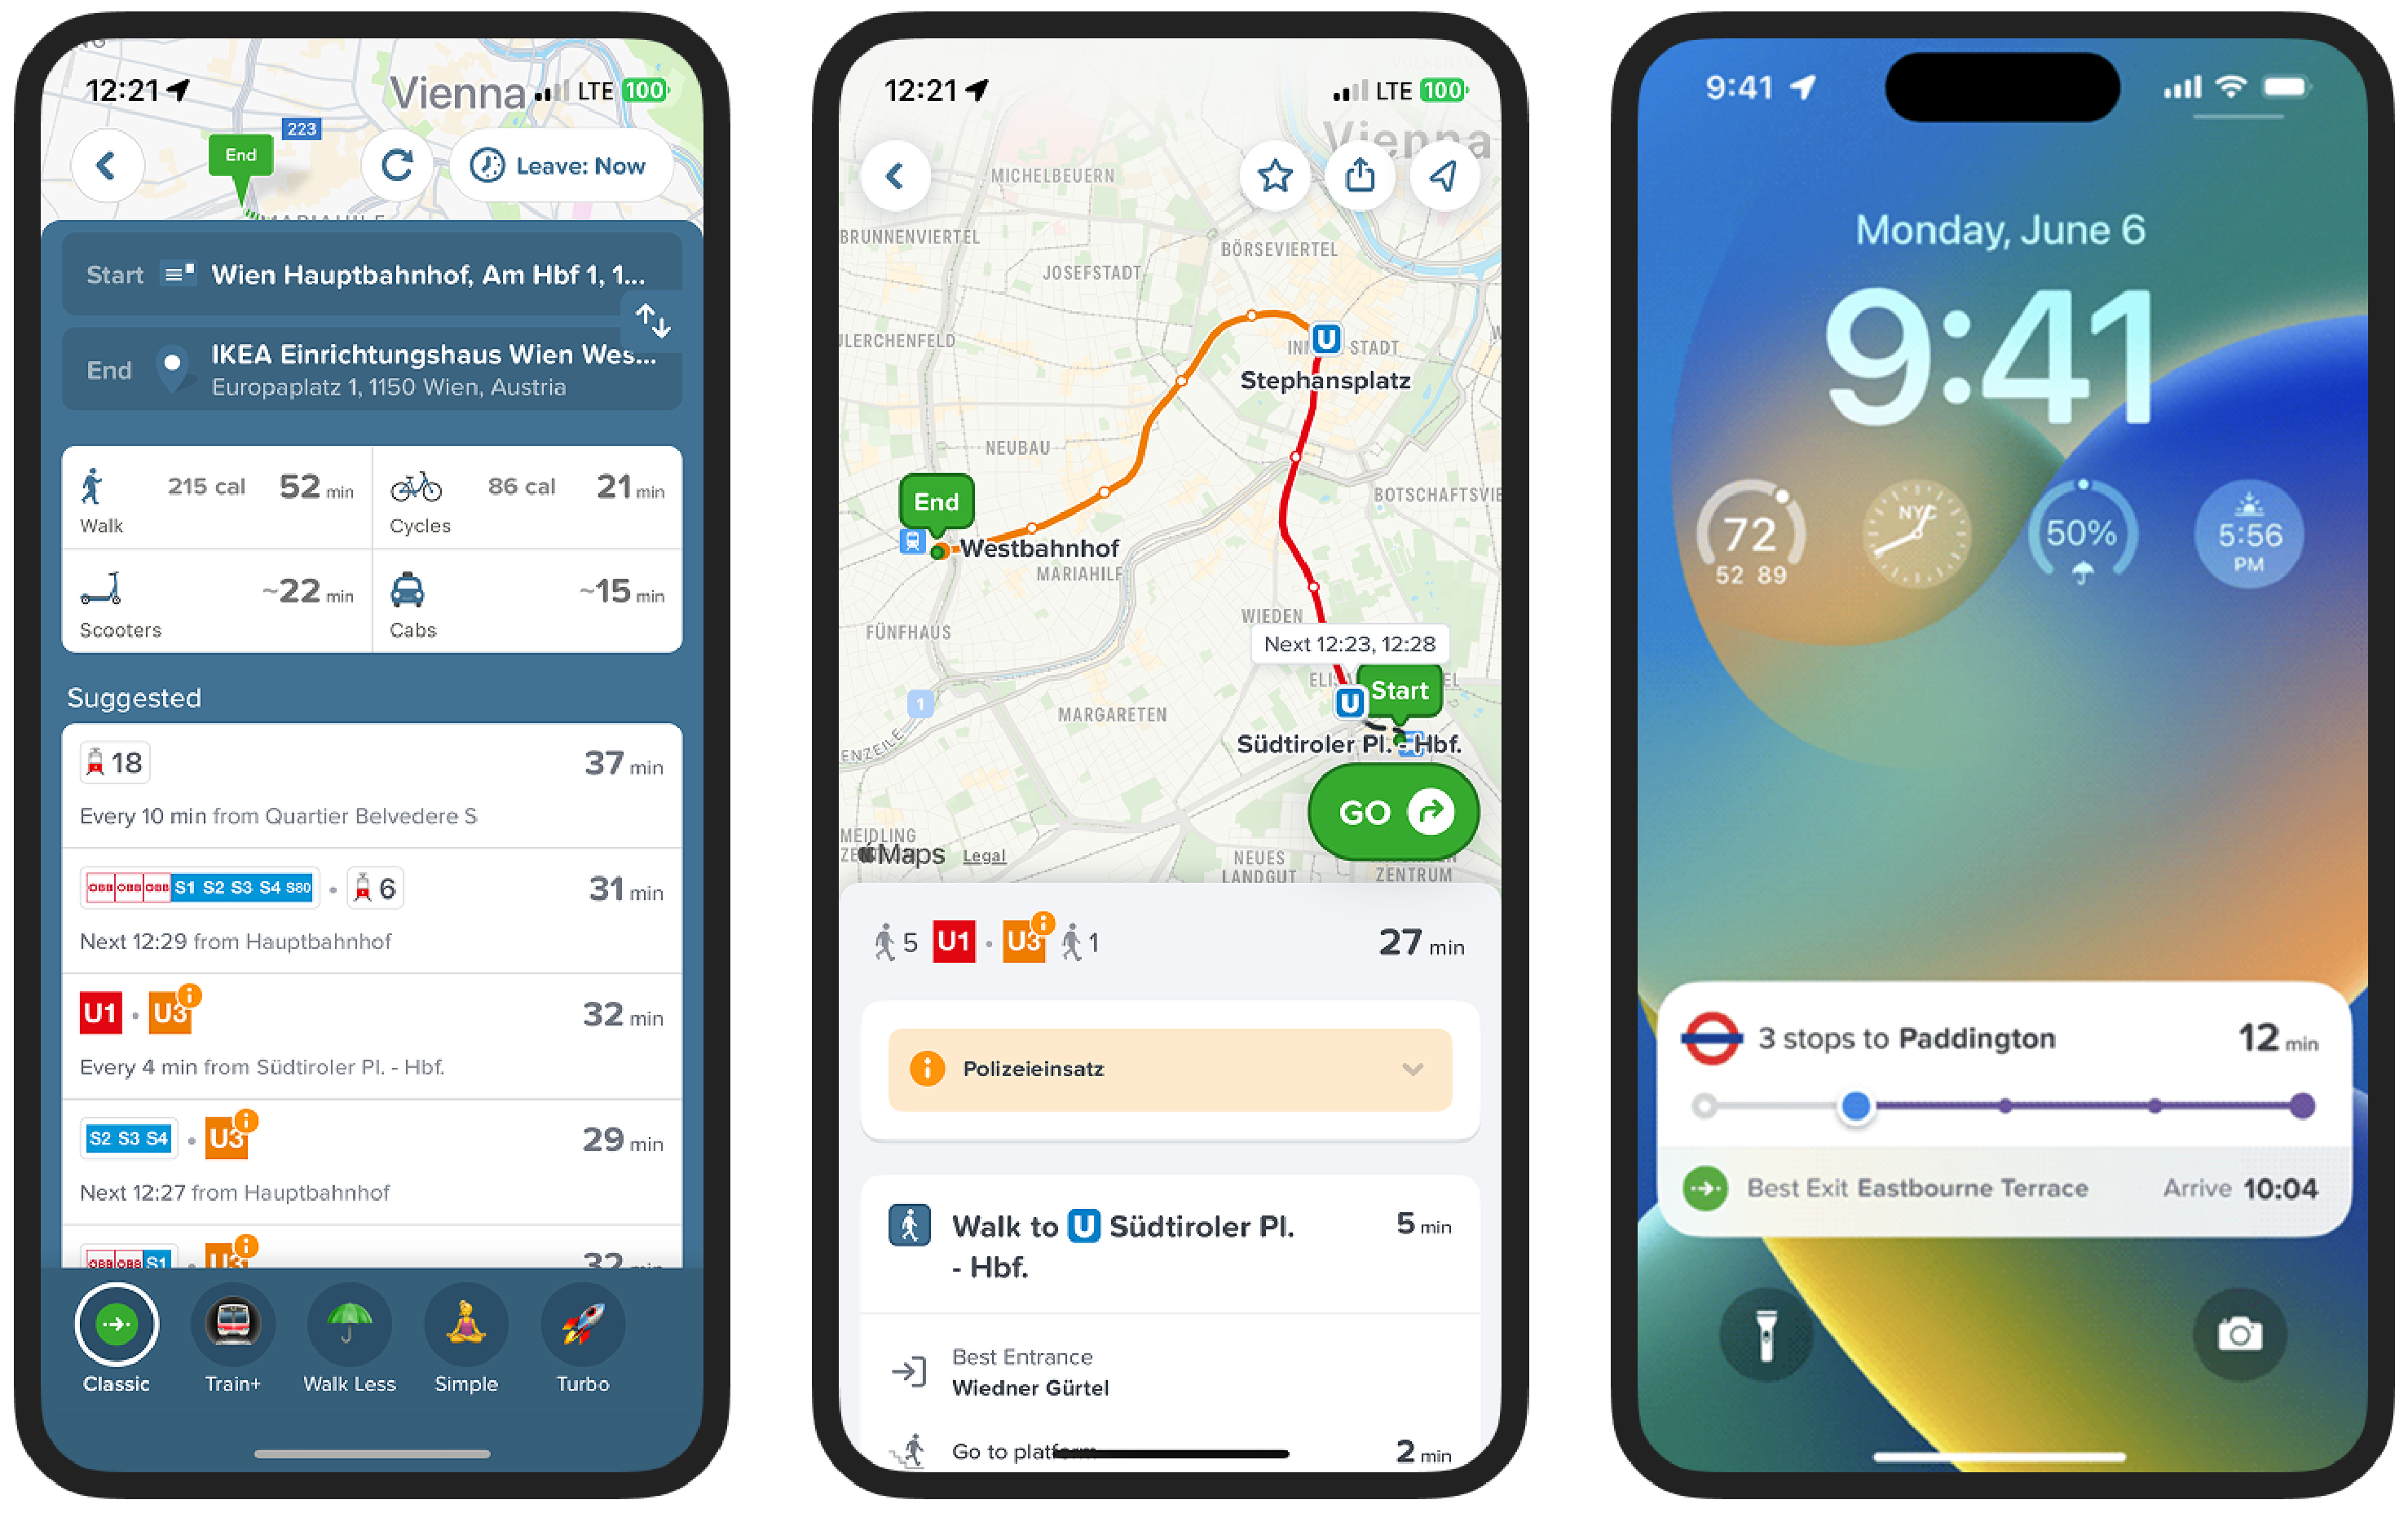
\includegraphics[width=0.7\textwidth]{Citymapper.pdf}
    \caption{Public transport route planning in the Citymapper app (left) and its Live Activity feature (right) \cite{citymapper_ios_lock_screen_navigation}}
    \label{fig:Citymapper}
\end{figure}

Moreover, the app allows users to track their CO$_2$ savings when using public transport, walking or cycling. 
It also provides the option to save favorite locations and label important places such as home and work for quick access. 
Additionally, calendar synchronization enables trip planning based on upcoming events and Siri integration allows users to receive commute updates via voice commands.
Alongside public transport routes, Citymapper integrates with ride-hailing services like Uber and Gett to provide fare estimates.

Citymapper has won Apple and Google's App of the Year awards multiple times and has over 50 million users worldwide.
The company briefly operated a night bus network in London to test transport alternatives. 
In 2023, Citymapper was acquired by Via, a company specializing in digital transit infrastructure.
This acquisition, as highlighted on Via's website \cite{via_acquires_citymapper}, suggests a shift in focus from a standalone tool to integration within a larger mobility ecosystem.
However, Via has stated that the acquisition will not impact the app's availability to its users and that they plan to expand its features and reach.

\section{Moovit}
Moovit is a public transportation navigation app launched in 2012 for iOS, Android and web browsers.
It aims to help users navigate cities by integrating multiple forms of transport including public transit, shared bikes, ride-hailing services such as Uber and Lyft, car-sharing and scooters into a single application.
Over the years, Moovit has grown significantly and now serves over 1.7 billion users in 3,500 cities across 112 countries and supports 45 languages, as stated on their website \cite{moovit_about}.

Moovit provides route planning and navigation as shown in in Figure~\ref{fig:Moovit} and displays nearby stops as well as arrival times for buses and trains.
Live tracking of transit lines and approaching line notifications are available through a premium subscription.
Other premium features include ad removal and traffic condition updates.
Users can save favorite locations, set home and work labels for quick access and sync their Apple Calendar for trip planning based on upcoming events.
Moovit also provides alerts for delays, service changes and reminders when to get off a bus or train.
The app includes a Way Finder feature, which uses augmented reality to help locate bus or train stops. 
Simlarily, commuters can upload photos to assist other users in recognizing stops or report station conditions and suggest updates to transit data.

\begin{figure}[htbp]
    \centering
    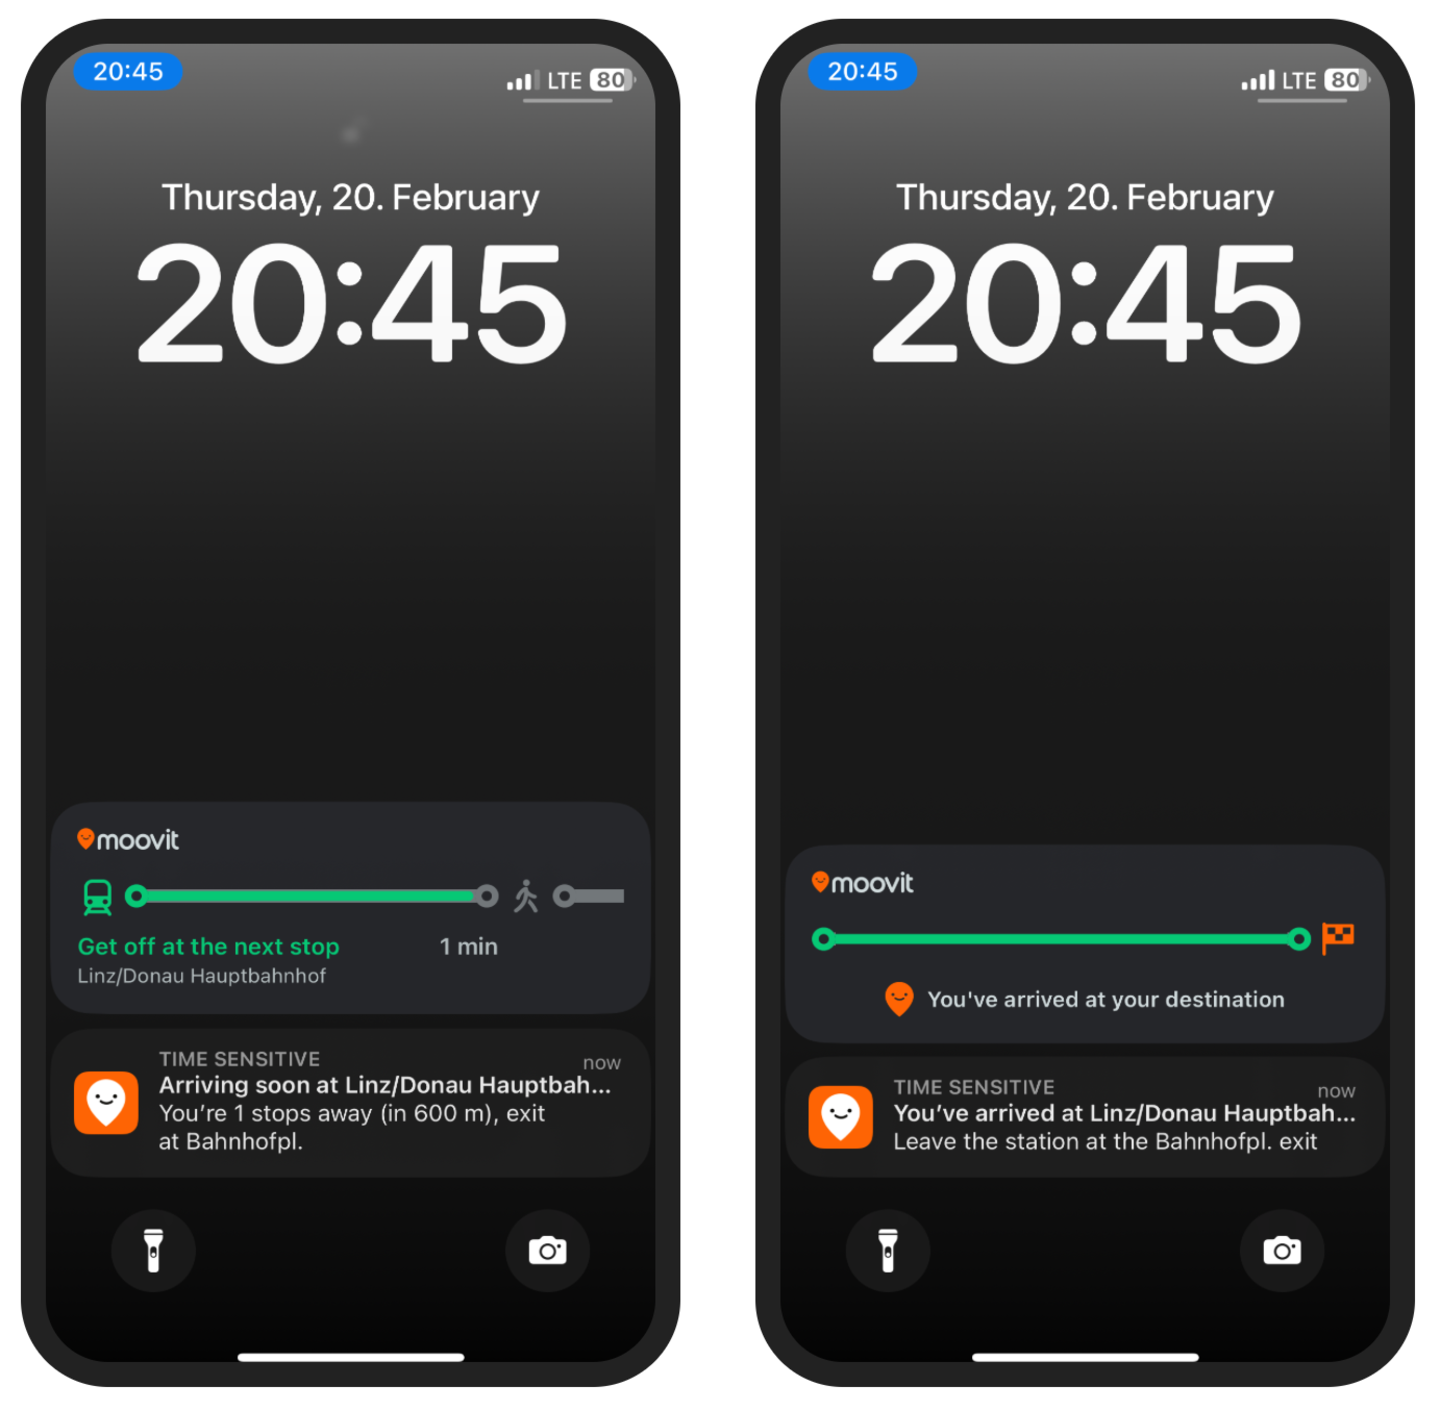
\includegraphics[width=0.7\textwidth]{Moovit.pdf}
    \caption{Public transport route planning and tracking in the Moovit app}
    \label{fig:Moovit}
\end{figure}

Moovit \cite{moovit_about} describes its transit data repository as one of the largest in the world. 
The app collects data from over 7,500 public transit operators and 360 micro-mobility providers and includes more than 6 million stops and stations.
However, a great part of its data collection comes from the Mooviter Community, a network of 875,000 local editors who contribute to updating transit information. 
This crowdsourced approach has helped Moovit expand to hundreds of new cities each year.
Since 2022, Moovit has been part of Mobileye to advance autonomous transportation solutions and it has received several awards such as Google's "Best Local App" in 2016 and Apple's "Best Apps of 2017".

\section{Conclusion}
The apps reviewed in this chapter all provide route planning and tracking, but they differ in how they notify users when to exit public transportation.
Google Maps offers Live Activities on iPhones which can show navigation updates on the lock screen. 
However, this feature is not consistently available and does not provide explicit stop notifications which means users must monitor their route on their own.
Citymapper goes a step further by offering "Get Off Alerts" in the form of notifications, which must be activated by the user.
Additionally, it provides Live Activities, similar to Google Maps, to help users track their journey progress.
Moovit also includes stop notifications, but none of the apps offer vibrational alerts or sound alarms, as proposed in this thesis.
The project aims to enhance user awareness by introducing a multi-step alert system, ensuring passengers receive both passive and active reminders when approaching their stop.
